\documentclass{standalone}
\usepackage[svgnames]{xcolor}
\usepackage{pgfplots}
\pgfplotsset{
    every axis/.append style={
        axis lines=middle,
        xlabel={$x$},
        ylabel={$y$},
        grid = both,
    }
}

\begin{document}
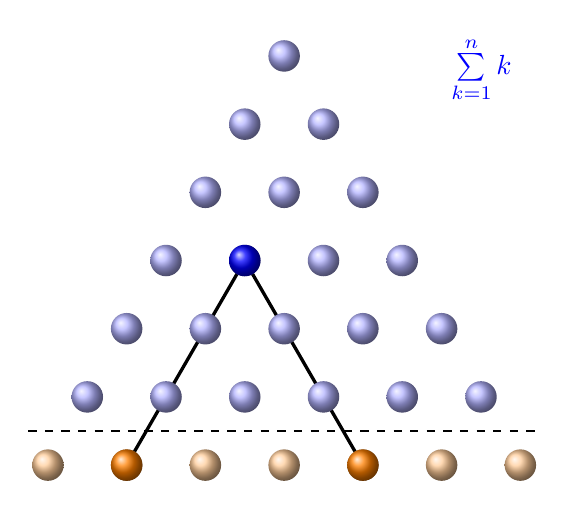
\begin{tikzpicture}
    \draw[dashed] (0.5-0.5*6.5,-0.866025*6.5) -- (7-0.5*6.5,-0.866025*6.5);
    \draw[very thick] (2-0.5*7,-0.866025*7) -- (2-0.5*4,-0.866025*4) -- (5-0.5*7,-0.866025*7);
    \foreach \x in {1,...,6}
        \foreach \y in {1,...,\x}
            \shade[ball color=blue!30] (\y-0.5*\x,-0.866025*\x) circle (0.2cm);
    \foreach \y in {1,...,7}
        \shade[ball color=orange!40] (\y-0.5*7,-0.866025*7) circle (0.2cm);
    \node at (2.5,-0.5) [anchor=north west]{\(\color{blue}\sum\limits_{k=1}^nk\color{black}\)};
    \shade[ball color=blue] (2-0.5*4,-0.866025*4) circle (0.2cm);
    \shade[ball color=orange] (2-0.5*7,-0.866025*7) circle (0.2cm);
    \shade[ball color=orange] (5-0.5*7,-0.866025*7) circle (0.2cm);
\end{tikzpicture}


\end{document}
